\chapter{АЛУ}

Арифметико-логическое устройство (АЛУ) компьютера отвечает за вычисления.
В современных компьютерах АЛУ находится внутри микропроцессора.
Чтобы что-то посчитать, процессор должен подключить ко входам АЛУ операнды
(из регистров или, к примеру, из выполняемой команды). Результат затем помещается
ещё в какой-то регистр.

% фиксированные входы-выходы

% фиксированный выход, отличающийся от входа

% произвольные входы-выходы

\section{Практикум}

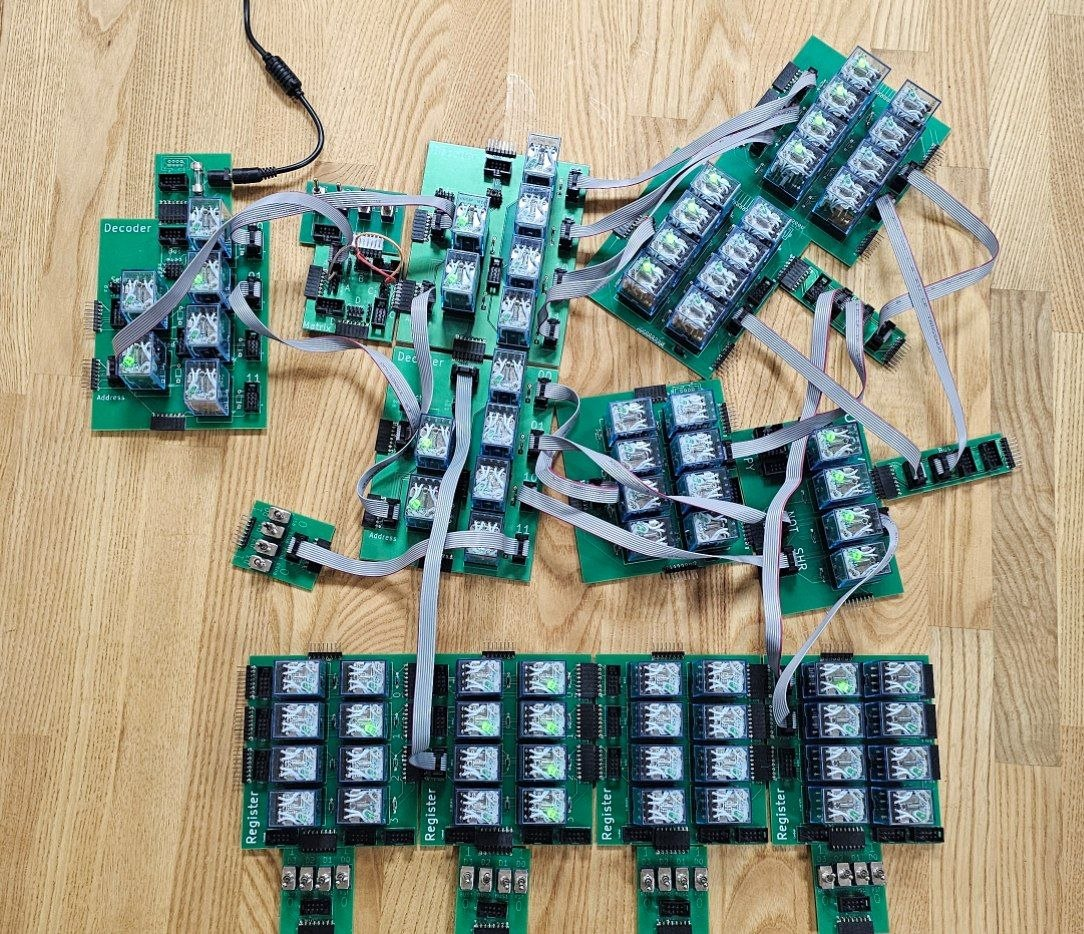
\includegraphics[width=\columnwidth]{photo/calculator3.jpg}

Калькулятор с выбором операндов из регистрового файла.

Список модулей:
\begin{itemize}
    \item Модуль переключателей: $6$ штук
    \item Модуль унарных операций: $1$ штука (или $2$ штуки)
    \item Сумматор: $2$ штуки
    \item Модуль логических операций: $1$ штука
    \item Дешифратор: $3$ штуки
    \item Регистровый модуль: $4$ штуки
    \item Кросс-модуль: $1$ штука
    \item Модуль шины: $2$ штуки
\end{itemize}


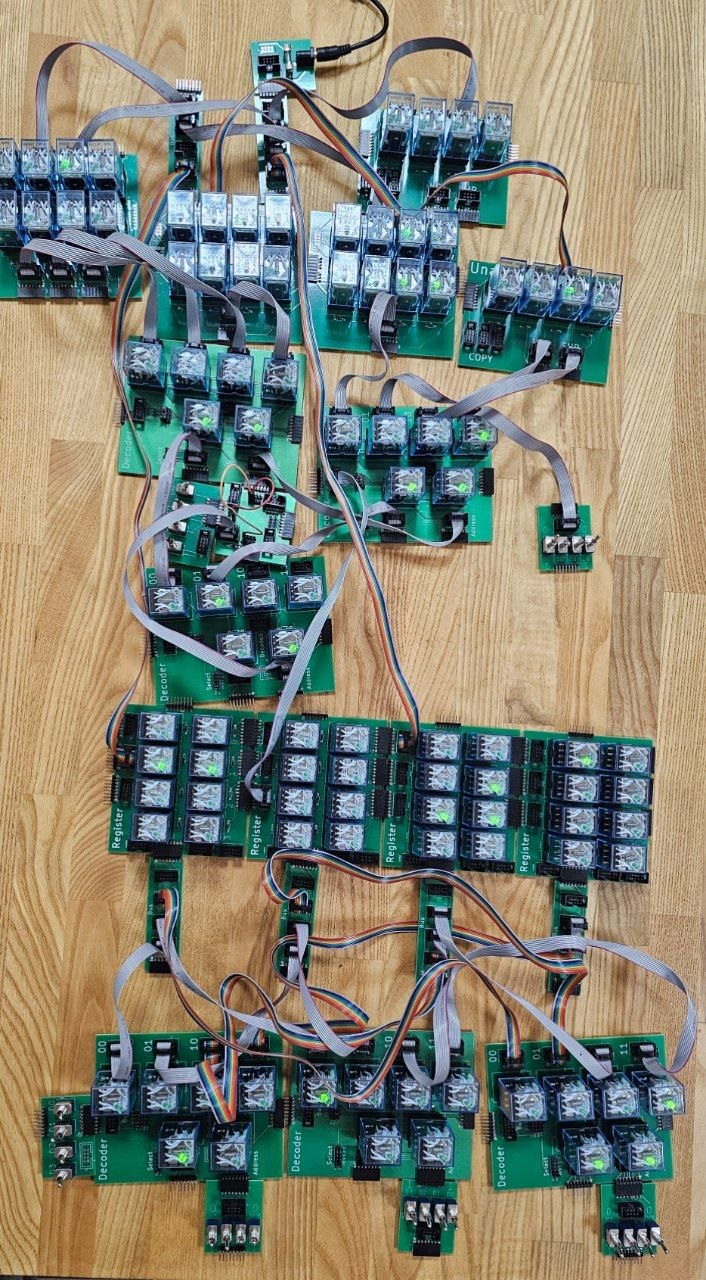
\includegraphics[width=\columnwidth]{photo/calculator4.jpg}

Калькулятор с выбором операндов из регистрового файла с помощью дешифраторов.

Список модулей:
\begin{itemize}
    \item Модуль переключателей: $6$ штук
    \item Модуль унарных операций: $1$ штука (или $2$ штуки)
    \item Сумматор: $2$ штуки
    \item Модуль логических операций: $1$ штука
    \item Дешифратор: $6$ штук
    \item Регистровый модуль: $4$ штуки
    \item Кросс-модуль: $1$ штука
    \item Модуль шины: $6$ штук
\end{itemize}
